\documentclass[12pt]{article}

\usepackage{ee143report}
\usepackage{verbatim}
\usepackage{graphicx, float}
\usepackage{enumerate}
\usepackage{amsmath}
\usepackage{bookmark}
\usepackage{pdflscape}
\usepackage{multirow}
\usepackage{hyperref}

\DeclareMathOperator{\V}{V}
\DeclareMathOperator{\A}{A}
\DeclareMathOperator{\F}{F}
\DeclareMathOperator{\mA}{mA}
\DeclareMathOperator{\mW}{mW}
\DeclareMathOperator\bit{bit}
\DeclareMathOperator\byte{byte}
\DeclareMathOperator\word{word}

\author{Astrid Yu}
\title{Arduino Ohmmeter}
\expNum{6}
\titlegraphic{
  \includegraphics[width=0.8\linewidth]{neither.jpg}
}

\begin{document}
\maketitle

\section*{Introduction}

In this experiment, an ohmmeter will be constructed from an Arduino. 
Code will be modified to improve the ohmmeter's measurements. 

\section*{Analysis}

\begin{enumerate}[a.]
    \item An Arduino was connected to a computer and the IDE was configured 
    to target the Arduino.
    \item The circuit shown in Figure \ref{fig:circuit} was built.
    \begin{figure}[H]
      \centering
      \includegraphics[width=0.5\linewidth]{circuit.png}
      \caption{The ohmmeter circuit.}
      \label{fig:circuit}
    \end{figure}
    
    \item The provided code was uploaded to the Arduino.
    \item The potentiometer was swept to various positions and the resistance was 
    measured to confirm the code worked.
    \item \textbf{Explain how the Arduino arrives at the R2 value displayed on the serial monitor.}
    
    The Arduino makes four measurements using the ADC so that the ADC can converge on a stable 
    value. Then, it uses various transformations based on knowledge about the circuit in order to 
    return the precise value. 
    \item A $4.3k\Omega\pm1\%$ resistor was measured using a digital multimeter to have 
    an actual resistance of $4.28k\Omega$.
    \item The potentiometer was replaced with the $4.3k\Omega$ resistor.
    \item The same resistor was measured using the Arduino Ohmmeter by pressing the button. 
    The results from the serial console are seen in Figure \ref{fig:meas1}
    \item The outputted value was $4267.78\Omega$.
    \begin{figure}[H]
      \centering
      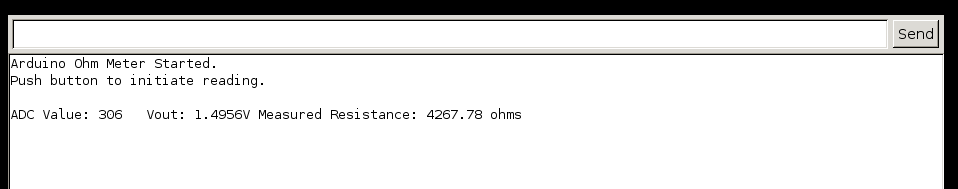
\includegraphics[width=\linewidth]{meas1.png}
      \caption{Arduino measurement of the resistor prior to calibration.}
      \label{fig:meas1}
    \end{figure}

    \item The error was calculated as follows: 
    \begin{equation}
        \begin{aligned}
            \frac{(\text{arduino measured}) - (\text{actual})}{(\text{actual})} \cdot 100 \% 
            &= \frac{4267.78\Omega - 4.28k\Omega}{4.28k\Omega} \cdot 100\% \\
            &= \mathbf{-0.303\%}
        \end{aligned}
    \end{equation}
    \item The 5V ADC reference is likely to be not exactly 5V. Additionally, the $10k\Omega$ 
    resistor has a non-zero tolerance on it. These variables could confound the measurement.
    
    The accuracy could be improved by compensating for the error by using this measurement 
    as a calibration measurement and multiplying the final result by a constant $k$ like so:
    \begin{equation}
        k\cdot (\text{arduino measured}) = (\text{actual})
    \end{equation}

    Solving for $k$ and plugging values in:
    \begin{equation}
        \begin{aligned}
            k &= \frac{(\text{actual})}{(\text{arduino measured})}  \\
            &= \frac{4.28k\Omega}{4267.78\Omega}  \\
            &= \mathbf{1.00286}
        \end{aligned}
    \end{equation}

    \item The code was modified to use this scaling constant.
    \item The recorded measurement was $4299.97\Omega$.
    The results from the serial console are seen in Figure \ref{fig:meas2}

    \begin{figure}[H]
      \centering
      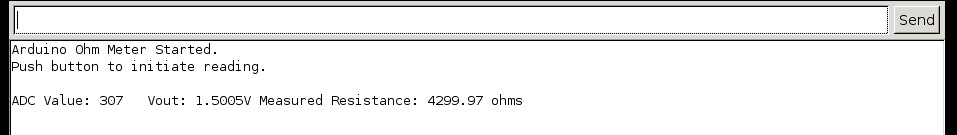
\includegraphics[width=\linewidth]{meas2.png}
      \caption{Arduino measurement of the resistor after calibration.}
      \label{fig:meas2}
    \end{figure}

    \item The error was calculated for this new measurement as follows:
    \begin{equation}
        \begin{aligned}
            \frac{(\text{arduino measured}) - (\text{actual})}{(\text{actual})} \cdot 100 \% 
            &= \frac{4299.97\Omega - 4.28k\Omega}{4.28k\Omega} \cdot 100\% \\
            &= \mathbf{+0.4666\%}
        \end{aligned}
    \end{equation}

    \item A red LED was added to the Arduino and the code was modified to turn the LED on when a short 
    is detected.
    \item A green LED was added to the Arduino and the code was modified to turn the LED on when 
    an open is detected. See Figures \ref{fig:neither}, \ref{fig:open}, and \ref{fig:short}.

    \begin{figure}[H]
      \centering
      \includegraphics[width=0.8\linewidth]{neither.jpg}
      \caption{The circuit with a load between the two electrodes. Note that neither LED is lit.}
      \label{fig:neither}
    \end{figure}
    \begin{figure}[H]
      \centering
      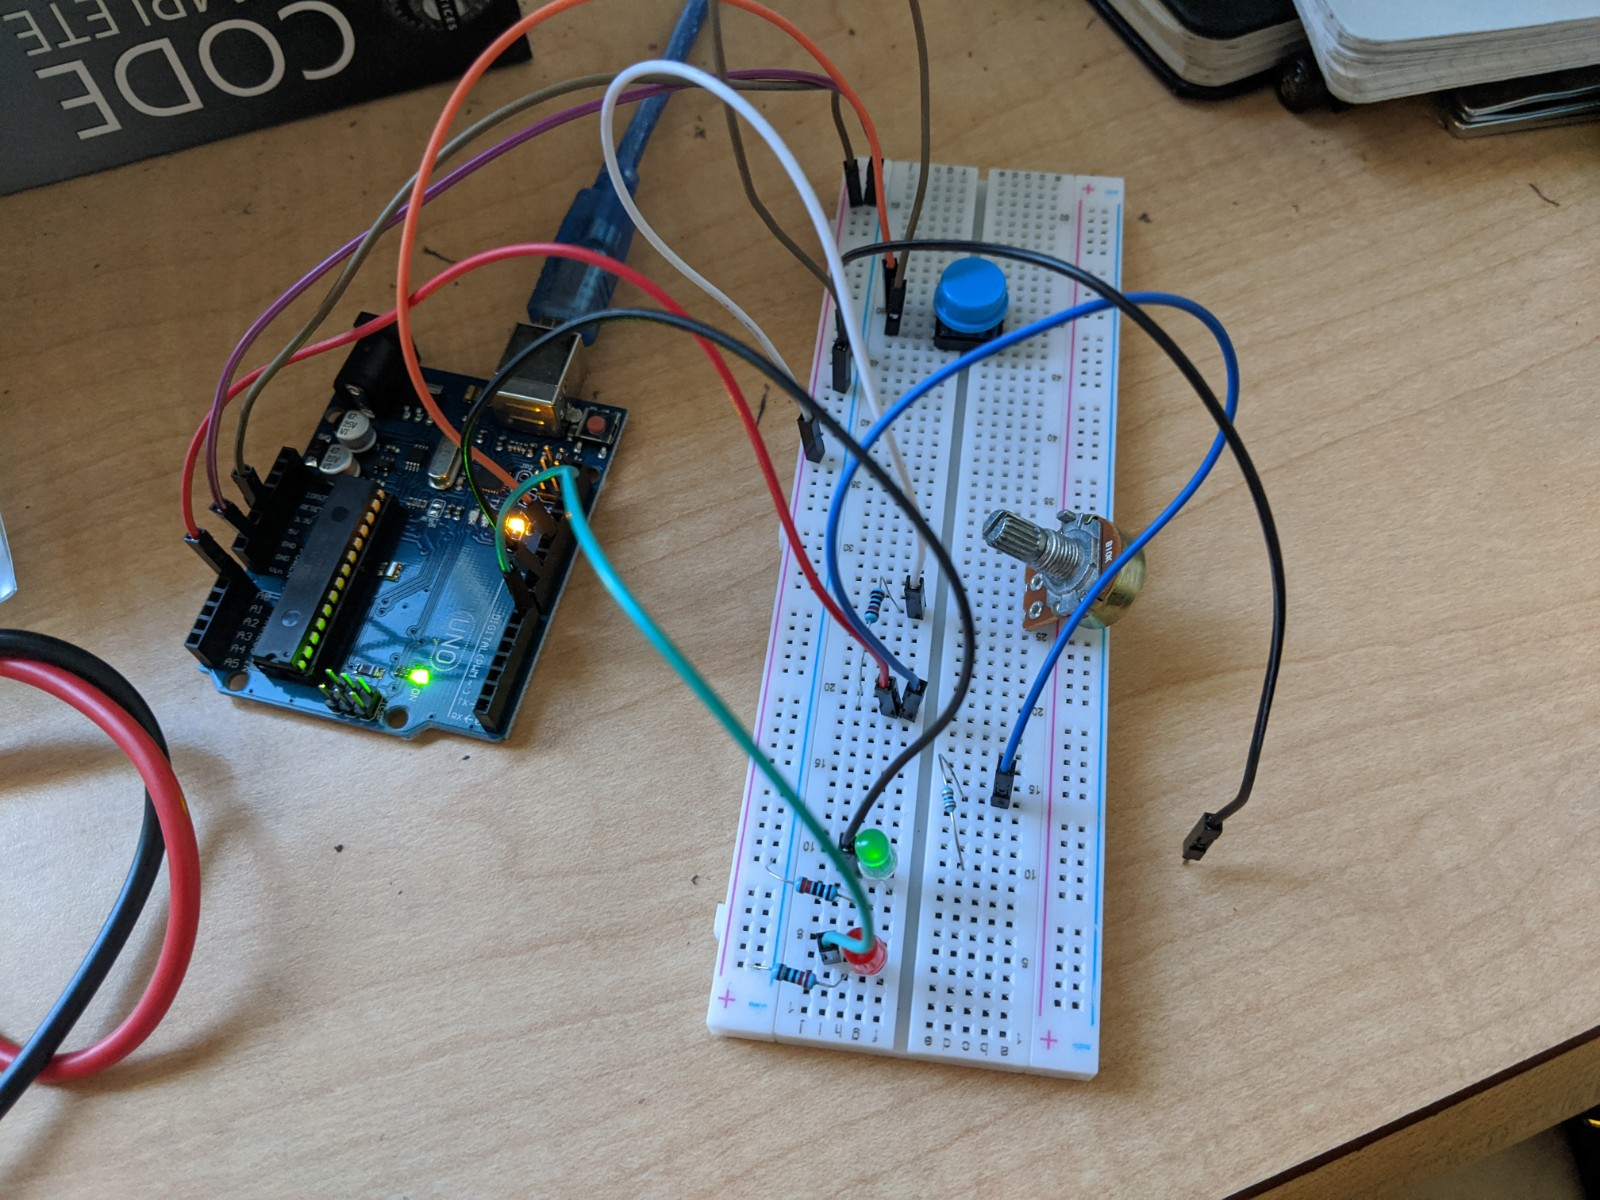
\includegraphics[width=0.8\linewidth]{open.jpg}
      \caption{The circuit in open position. Note the green LED being lit, albeit dimly.}
      \label{fig:open}
    \end{figure}
    \begin{figure}[H]
      \centering
      \includegraphics[width=0.8\linewidth]{short.jpg}
      \caption{The circuit with a short. Note the red LED being lit.}
      \label{fig:short}
    \end{figure}
\end{enumerate}

\section*{Discussion Questions}

\begin{enumerate}
    \item The second time, a positive error was produced, and not only that, the error is even greater. 
    This may be because the Arduino's readings are not only less accurate, but less precise. Only one 
    calibration measurement was produced when it would probably better to make a few hundred. It is likely 
    that the calibration measurement may have been a low outlier, causing the formula to overcompensate.

    \item The source code begins on the next page.
\end{enumerate}

\pagebreak

\subsection*{Modified Source Code}

\begin{verbatim}
#include <Bounce2.h> 

#define LED_OPEN 9
#define LED_SHORT 7

const float Vin = 5.0;  //should start with Vin = 5.0
const float R1 = 10000; //should start with R1 = 10K
const int CIRCUIT = 0; //using analog input A0
const int BUTTON = 12; //Button to ground on pin 12
const int READ_DELAY_mS = 1; //delay between successive reads

//4.89 mV / ADC count, assuming 5V reference
const float VOLTS_PER_COUNT = Vin/1023.0; 


Bounce Button = Bounce(); //Button object from Bounce library
float Vout; //voltage out of voltage divier, read by ADC
char VoutString[100]; //string representation of Vout
float R2; //"unknown" resistance
int ADCvalue; // value read from ADC

void setup() {
  // serial monitor used at 115200 bps
  Serial.begin(115200);
  // trigger button
  pinMode(BUTTON, INPUT_PULLUP);
  // using the Bounce2 library to debounce the button
  Button.attach(BUTTON,INPUT_PULLUP);
  Button.interval(25);
  // starting salutation
  Serial.println("Arduino Ohm Meter Started.");
  Serial.println("Push button to initiate reading.");
}

void loop() {
  // Is the button pushed?
  Button.update();
  bool ButtonPushed = !Button.read(); // invert logic to true = pushed
  
  // if the button is pushed, generate a reading
  if (ButtonPushed) {
    //read the ADC four times to get a stable reading
    for (int i=0; i < 4; i++) {
      ADCvalue = analogRead(CIRCUIT);
      delay(READ_DELAY_mS);
    }
    //calculate the voltage that was read
    Vout = (float)ADCvalue * VOLTS_PER_COUNT;
    // calculate the resistance
    R2 = 1.00286 * (Vout*R1)/(Vin-Vout);
    // print the results to the serial monitor
    Serial.print("ADC Value: ");
    Serial.print(ADCvalue);
    Serial.print("   Vout: ");
    dtostrf(Vout, 1,4, VoutString);
    Serial.print(VoutString);
    Serial.print("V");
    Serial.print(" Measured Resistance: ");
    Serial.print(R2);
    Serial.println(" ohms");
    // wait for the button to be released before proceeding
  }

  int continuityMeasurement = analogRead(CIRCUIT);
  bool openState = 0;
  bool shortState = 0;
  if (continuityMeasurement == 1023) {
    openState = 1;
  } else if (continuityMeasurement == 0) {
    shortState = 1;
  }
  digitalWrite(LED_OPEN, openState);
  digitalWrite(LED_SHORT, shortState);
  
  while (ButtonPushed) {
    Button.update();
    ButtonPushed = !Button.read();
  }
}
\end{verbatim}

\pagebreak

\section*{Conclusion}

In this experiment, a digital ohmmeter was successfully constructed and tested.
Attempts were made to improve the readings were not successful, likely 
due to a small sample size. In a future experiment or in a production 
environment, more measurements would need to be made and analyzed to 
ensure accuracy and precision together.

\end{document}
